
\section{Investigating Gain Using Magnitude Estimation}
\label{sec-rq3}

The previous section used perturbations in system orderings to examine
the difference between using magnitude estimate relevance scores and
the usually employed ordinal relevance levels as gains.
This section directly considers gain profiles, answering our fourth
research question RQ\ref{item:rq3} by considering what additional
insights magnitude estimation can provide into user perceptions of
relevance.


\begin{figure}[t]
  \centering
  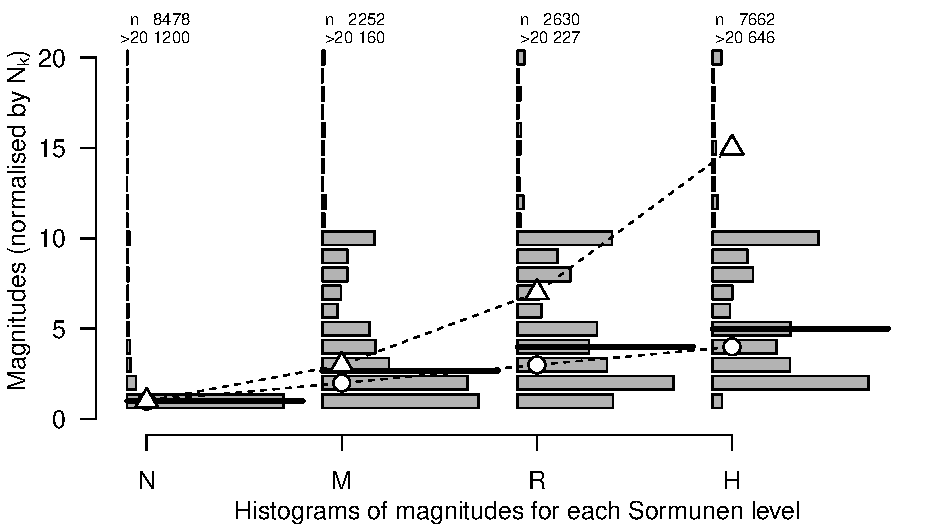
\includegraphics[width=.7\linewidth]{figs/gains_ratios_all.pdf}
  \caption{Distribution of magnitudes (normalized by \nkn) for each Sormunen level.
    Circles are linear gain values, $\{1,2,3,4\}$, while triangles 
    represent exponential gain values, $\{2^1,2^2,2^3$,$2^4\}$.
    Black lines are medians; the text ``n'' gives the total number of magnitudes in the level, and ``$>20$'' shows
    the count of scores above 20.
  \label{fig:ratio-gain-values}
  }
\end{figure}


The gain weights of the nDCG metric allow for the modeling of
different user relevance preferences.
However, in practice gains are usually set to one of two profiles: a 
\emph{linear} setting (as defined in Section~\ref{sec:rq2}); or an
\emph{exponential} setting, where the ordinal relevance level
forms a power of 2~\cite{BurSha05}, placing more emphasis on highly
relevant documents.
Figure~\ref{fig:ratio-gain-values} shows the distribution of magnitude
estimation scores, normalized by the \nkn score in each unit (intuitively,
a measure of relevance standardized for each user).
Black lines show the median magnitudes for each group.
Superimposed are the two default profiles, linear (white circles), and
exponential (white triangles).
It can be seen that, compared to actual user perceptions of the
relevance space, the linear gain profile is fairly close to 
the gain that should be allocated at each level to satisfy the
(mythical) median user.
The exponential profile is further from the median, overestimating the
gain for the \rr and \hh levels, but catering for some judgments.

It is readily apparent, however, that the large spread of the 
distributions of
magnitudes cannot be captured in a single gain formulation.
There is simply too much individual variation to warrant the
simplification of relevance perceptions to a single profile.

\citet{KanAsl03} investigated how gain values could be set in nDCG so
as to maximize the stability of system rankings, based on the
generalizability and dependability coefficients from Generalizability
Theory.
The settings were estimated empirically, based on system runs from the
TREC 9 and 10 Web Tracks and the TREC 12 Robust Track.
We compare this approach with ME scores of relevance perceptions
gathered from users.
Figure~\ref{fig:ka} shows the ratio of magnitudes for document pairs in
the Sormunen categories highly relevant and partially relevant.
The ratios are computed within each unit collected (8 documents for one
topic), and if the unit contains more than one document in some
category, all combinations of the documents are included in the graph.
To allow comparison with gain values recommended by 
\citet{KanAsl03}, we either ignore marginally 
relevant documents (Sormunen category M), leftmost box; fold them in as
partially relevant, middle box; or call them partially relevant and
promote category R to highly relevant.
When a unit did not contain a marginally relevant document, it is
omitted from the middle and right boxes, hence there are less grey dots
for those plots.

Kanoulas and Aslam~\cite{KanAsl03} recommend a ratio of 1.1 for the
gain values of relevant to highly relevant documents to maximize the
effectiveness of a system comparison experiment.
Using magnitudes directly as gain values gives a median of 1.00, 1.00,
and 1.14 in the three boxes in Figure~\ref{fig:ka}, which happens to be
close to their recommendation.
However, again, we see a wide variation from this median, and mean
values of the ratios are 48, 22 and 24 respectively, further suggesting
that there may not be a single gain setting that is suitably
representative across different user perceptions and tasks.
% This hints that using median aggregation might be best for maximizing the statistical efficiency of system
% comparisons using magnitudes as gain values.
% \aht{Really - does this last sentence even make logical senes? median of ratios matches, so use median
% aggregation???}

\begin{figure}[t]
  \centering
  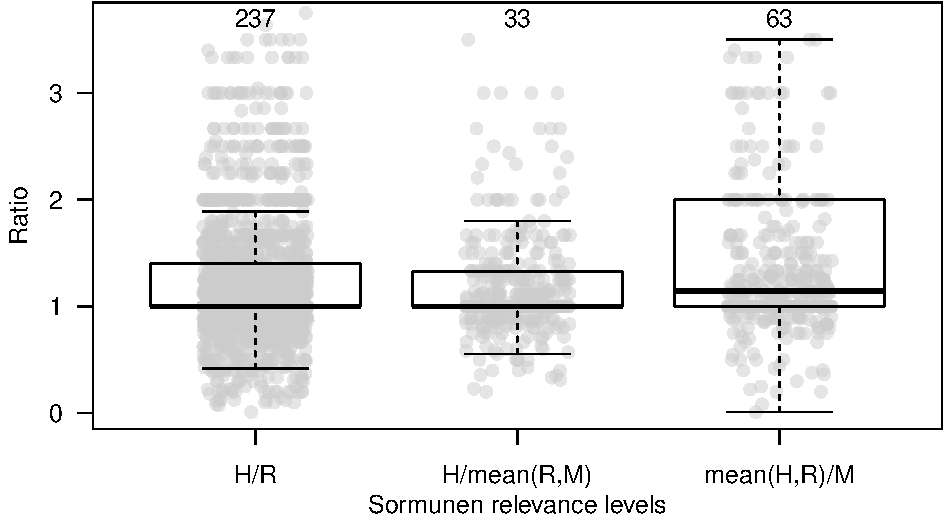
\includegraphics[width=.7\linewidth]{figs/kanoulos_aslam.pdf}
  \caption{Ratio of the magnitude scores assigned to 
    the Sormunen categories highly relevant (H) to relevant (R) and marginally relevant
    (M) over all pairs of documents. Numbers indicate the count of document pairs that 
    are greater than 3.5 for each box. Each grey dot is a ratio of one document pair.
  \label{fig:ka}
    }
\end{figure}

\subsection{Summary}

\textcolor{red}{
In the previous section, and in this section, we have seen not only 
that relevance values for a single document vary amongst users, but
the ratio of relevance between two documents also varies.
Thus, in answer to RQ\ref{item:rq3}, the selection of a single 
gain formulation as either
a linear or exponential mapping of categorical judgements
is guaranteed to misrepresent at least half of our users 
in this data set.
Similarly, choosing a single gain formulation to maximize statistical 
efficiency of system comparisons will also misrepresent a large 
part of the user population.
}




% Local Variables:
% TeX-master: "ME-TOIS.tex"
% End:
